\section{Creating your PGP keys}

Enigmail comes with a nice wizard to help you create a public/private
key pair (see the chapter introducing PGP for an explanation). You can
start the wizard at any time within Thunderbird by selecting
\verb!OpenPGP > Setup Wizard! from the menu on top.

\begin{enumerate}[1.]
\item
  This is what the wizard looks like. Please read the text on every
  window carefully. It provides useful information and helps you setup
  PGP to your personal preferences. In the first screen, click on Next
  to start the configuration.
\end{enumerate}
\begin{figure}[htbp]
\centering
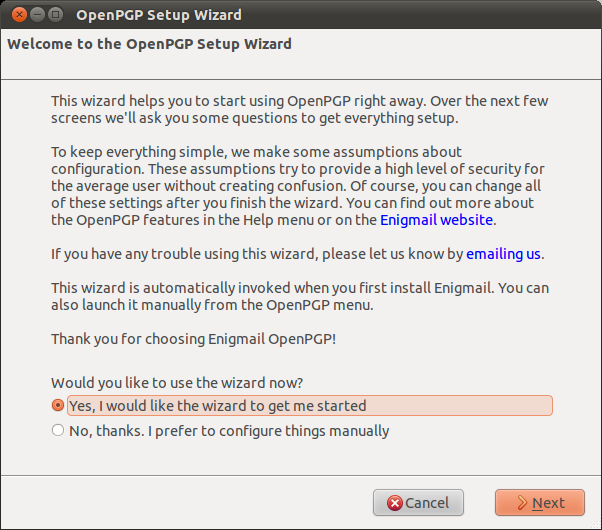
\includegraphics{gpg_keys_1.png}
\caption{GPG Keys}
\end{figure}

\begin{enumerate}[1.]
\setcounter{enumi}{1}
\item
  The wizard asks you whether you want to sign all your outgoing mail
  messages. Signing all your messages is a good choice. If you choose
  not to, you can still manually decide to sign a message when you are
  composing it. Click on the `Next' button after you have made a
  decision.
\end{enumerate}
\begin{figure}[htbp]
\centering
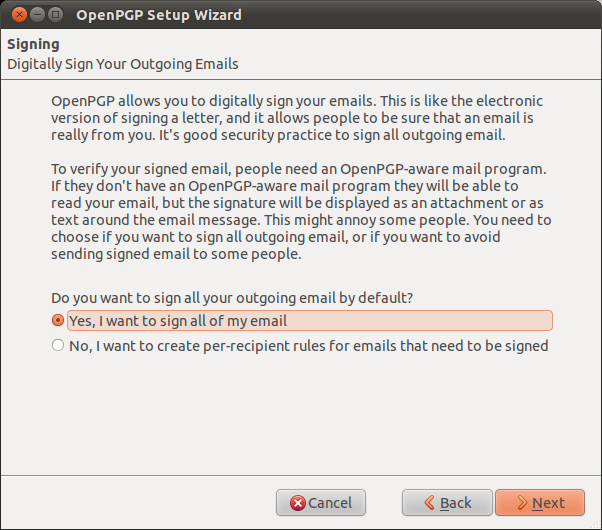
\includegraphics{gpg_keys_2.png}
\caption{GPG Keys}
\end{figure}

\begin{enumerate}[1.]
\setcounter{enumi}{2}
\item
  On the following screen, the wizard asks you whether you want to
  encrypt \emph{all} your outgoing mail messages. Unlike signing of
  mails, encryption requires the recipient to have PGP software
  installed. You should probably answer `no' to this question, so that
  you will send normal (unencrypted) mail by default. After you have
  made your decision, click on the `Next' button.
\end{enumerate}
\begin{figure}[htbp]
\centering
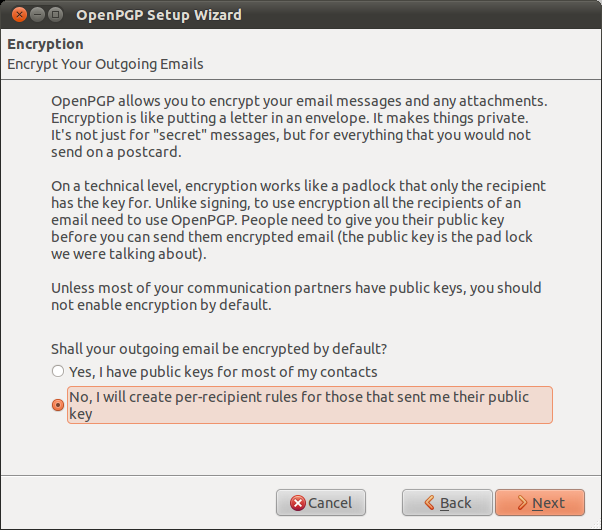
\includegraphics{gpg_keys_3.png}
\caption{GPG Keys}
\end{figure}

\begin{enumerate}[1.]
\setcounter{enumi}{3}
\item
  On the following screen the wizard asks if it can change some of your
  mail formatting settings to better work with PGP. It is a good choice
  to answer `Yes' here. This will mean that by default, mail will be
  composed in plain text rather than HTML. Click on the `Next' button
  after you have made your decision.
\end{enumerate}
\begin{figure}[htbp]
\centering
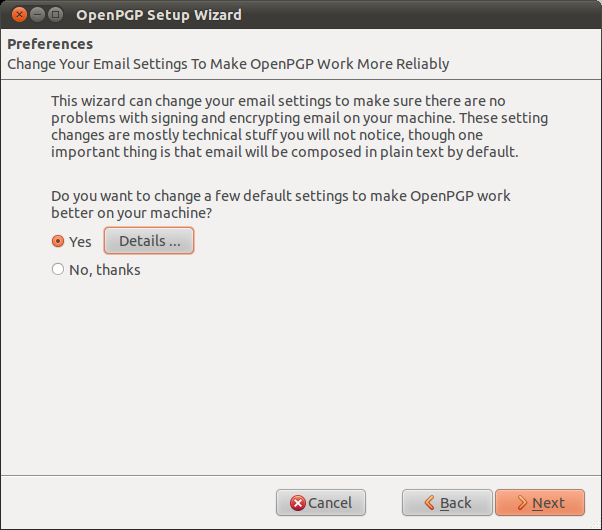
\includegraphics{gpg_keys_4.png}
\caption{GPG Keys}
\end{figure}

\begin{enumerate}[1.]
\setcounter{enumi}{4}
\item
  In the following screen, select one of your mail accounts; the default
  is selected for you if you only have one. In the `Passphrase' text box
  you must enter a password. This is a \emph{new} password which is used
  to protect your private key. It is \textbf{very important} to remember
  this password, because you cannot read your own encrypted emails if
  you forget it. Make it a \textbf{strong} password, ideally 20
  characters or longer. Please see the chapter on passwords for help on
  creating unique, long and easy to remember passwords. After you have
  selected your account and created a passphrase, click on the `Next'
  button.
\end{enumerate}
\begin{figure}[htbp]
\centering
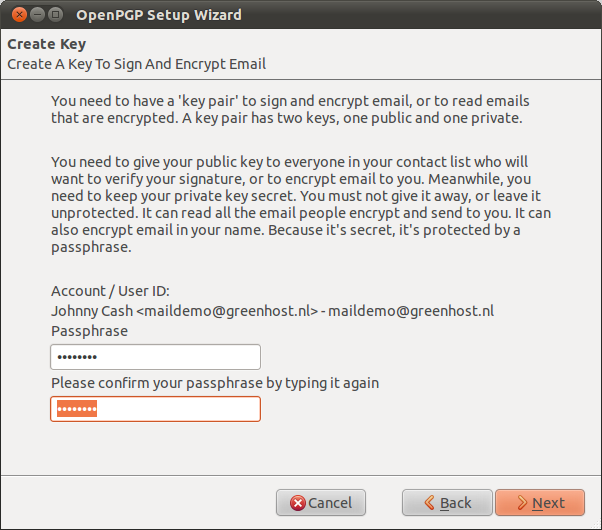
\includegraphics{gpg_keys_5.png}
\caption{GPG Keys}
\end{figure}

\begin{enumerate}[1.]
\setcounter{enumi}{5}
\item
  In the following screen the wizard summarizes the actions it will take
  to enable PGP encryption for your account. If you are satisfied, click
  the `Next' button.
\end{enumerate}
\begin{figure}[htbp]
\centering
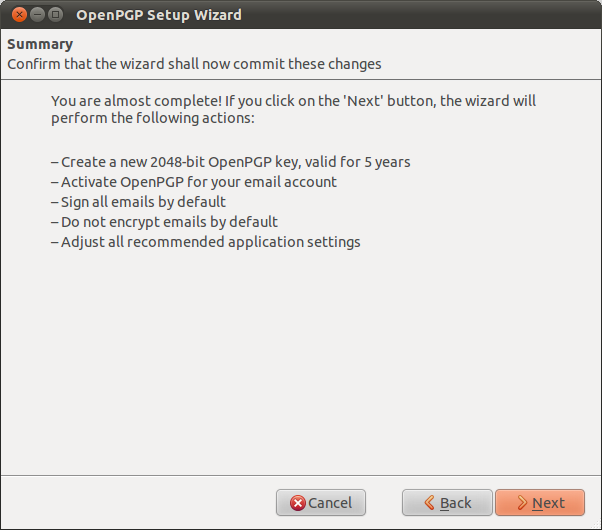
\includegraphics{gpg_keys_6.png}
\caption{GPG Keys}
\end{figure}

\begin{enumerate}[1.]
\setcounter{enumi}{6}
\item
  Your keys will be created by the wizard, which will take some time.
  When completed, click on the `Next' button.
\end{enumerate}
\begin{figure}[htbp]
\centering
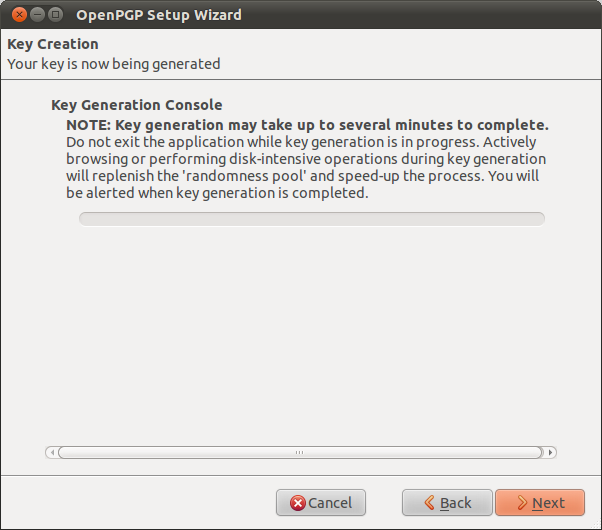
\includegraphics{gpg_keys_7.png}
\caption{GPG Keys}
\end{figure}

\begin{enumerate}[1.]
\setcounter{enumi}{7}
\item
  You now have your own PGP key-pair. The wizard will ask you if you
  also want to create a `Revocation certificate'. This is a file which
  can be used to inform everyone if your private key is compromised, for
  example if your laptop is stolen. Think of it as a `kill switch' for
  your PGP identity. You may also wish to revoke the key simply because
  you have generated a new one, and the old one is obsolete.
\end{enumerate}
\begin{figure}[htbp]
\centering
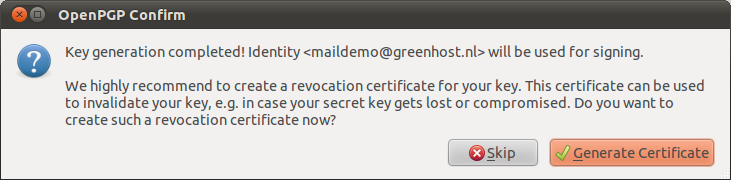
\includegraphics{gpg_keys_8.png}
\caption{GPG Keys}
\end{figure}

\begin{enumerate}[1.]
\setcounter{enumi}{8}
\item
  If you decided to generate a revocation certificate, the wizard will
  ask you where the file should be saved. The dialog will look different
  depending on which operating system you use. It is a good idea to
  rename the file to something sensible like
  my\_revocation\_certificate. Click on `Save' when you you have decided
  on a location.
\end{enumerate}
\begin{figure}[htbp]
\centering
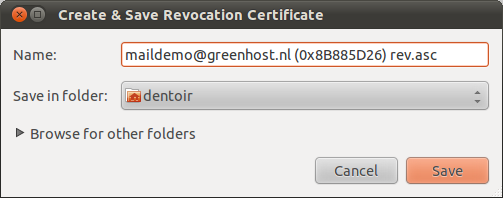
\includegraphics{gpg_keys_9.png}
\caption{GPG Keys}
\end{figure}

\begin{enumerate}[1.]
\setcounter{enumi}{9}
\item
  If you decided to generate a revocation certificate, the wizard
  informs you it has been successfully stored. You may want to print it
  out or burn it to a CD and keep it in a safe place.
\end{enumerate}
\begin{figure}[htbp]
\centering
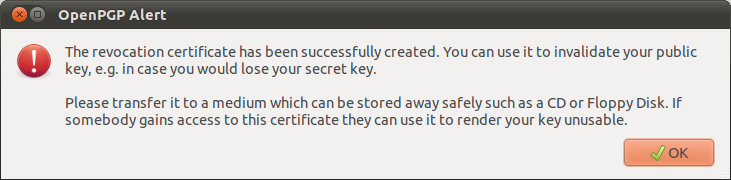
\includegraphics{gpg_keys_10.png}
\caption{GPG Keys}
\end{figure}

\begin{enumerate}[1.]
\setcounter{enumi}{10}
\item
  The wizard will inform you it has completed.
\end{enumerate}
\begin{figure}[htbp]
\centering
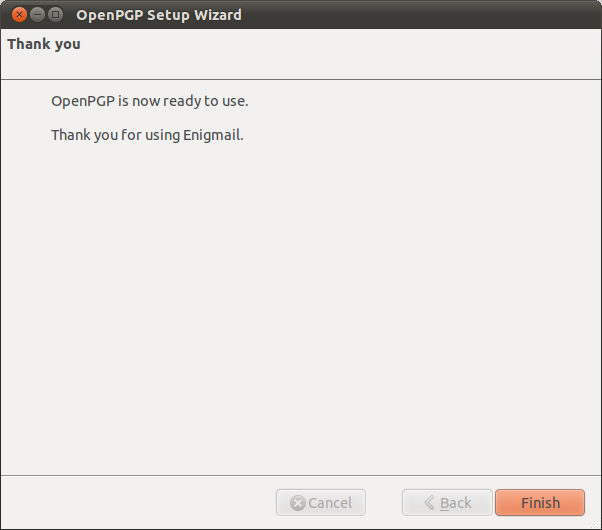
\includegraphics{gpg_keys_11.png}
\caption{GPG Keys}
\end{figure}

Congratulations, you now have a fully PGP-configured mail client. In the
next chapter we will explain how to manage your keys, sign messages and
do encryption. Thunderbird can help you do a lot of these things
automatically.
